\subsection{Detalls d'implementació}

    \paragraph{}
    Abans de destacar els detalls d'implementació d'aquesta funcionalitat, volem comentar, de la mateixa forma que per les dues funcionalitats anteriors, que només el controlador que gestiona la funcionalitat, està format per tres-centes línies de codi i en conseqüència, manca de sentit intentar representar totes les funcionalitats i aspectes d'aquesta en la memòria.

    El controlador encarregat del funcionament de l'evolució temporal d'esdeveniments és el fitxer \emph{facts.js}.

    \subsubsection{Validació del formulari de cerca}

\paragraph{}
A diferència de la funcionalitat de cerca general, aquesta funcionalitat, sí que realitza una validació més exhaustiva dels valors introduïts per l'usuari a través del formulari, ja que una configuració incorrecta d'aquests, resultaria l’obtenció de zero resultats.

    \subsubsection{Regulació de les crides asíncrones}

\paragraph{}
De la mateixa forma que la funcionalitat expansió geogràfica d’un cognom, aquesta funcionalitat llança múltiples crides asíncrones contra el SDK de FamilySearch.

En concret, aquesta funcionalitat, sempre llença onze crides que per evitar ser bloquejades per la funcionalitat de `throttling' de l’API de FamilySearch, han estat serialitzades imposant una pausa de dos segons i mig entre crida i crida.

Aquesta serialització s'ha aconseguit, de forma anàloga a la descrita en detall a la funcionalitat anterior, mitjançant la funció \emph{setTimeout()} de jQuery i el paràmetre \emph{apiDELAY}, que s'encarrega d'indicar l'interval d'espera entre les diferents crides. També s'han encapsulat les crides en una funció, que emmagatzema com a paràmetre a quina de les onze crides correspon la iteració.

A continuació, mostrem el bloc de codi reduït, que representa la serialització de les crides a l’API.

\begin{lstlisting}[style=rawOwn,caption={Separació manual de les crides asíncrones al SDK}]
for(var i = 0; i < 11; i++) {
    ...
    (function(i) {
        setTimeout(function() {
            ...
            client.getPersonSearch(params).then(function(searchResponse) {
            var total = searchResponse.getResultsCount();
            linechartRows[i].push(String(firstYear+i));
            linechartRows[i].push(total);
            ...
            });
        }, apiDELAY*i);
    }(i));
}
\end{lstlisting}

Aquestes crides retornen al controlador una per una i encara que no podem garantir l'ordre de rebuda, s’espera que en la gran majoria dels casos, aquest es correspongui a l’ordre d’enviament. De totes maneres, gràcies al paràmetre \emph{i}, empaquetat en cada una de les crides, podem emmagatzemar les dades retornades pel SDK al lloc que els hi correspon de la matriu \emph{linechartRows}.

La variable global encarregada de guardar els resultats de les diferents crides al SDK és la mateixa que la utilitzada pel gràfic de línies de la funcionalitat expansió geogràfica d'un cognom, però que en aquest cas, consisteix en una matriu d'una sola columna, on la columna representa la localització cercada i cada fila, el valor per un any concret.

Explicar que utilitzem una matriu d'una sola columna, en comptes d'un vector, perquè aquest és el format que espera l'API de Google, si volem que el gràfic representi la quantitat d'instàncies trobades en l'eix vertical i els anys a l'eix horitzontal.

La línia de codi responsable de guardar els valors per cada crida a l’API, ha estat mostrada en el bloc de codi anterior i en concret, a les files vuit i nou. Recordem, que el paràmetre \emph{i} fa referència a la iteració del bucle executada i per extensió, a quin any fan referència les dades respecta els onze anys de l’interval cercat.

    \subsubsection{Impressió dels gràfics}

\paragraph{}
A causa de la funcionalitat, resulta fàcil, que a la mínima que es realitza una cerca interessant, aquesta tardi més d'un minut en completar-se.

Per tal de transmetre la sensació de moviment i que el sistema està treballant, hem introduït a la funcionalitat la capacitat d'anar pintant els gràfics de cada any, a mesura que les dades van quedant disponibles. És a dir, que no cal esperar fins al final de la cerca per poder començar a veure resultats.

Per aconseguir aquest efecte, disposem de variables globals que comptabilitzen el nombre de cerques que ja han retornat del SDK i cada cop que les dades d'un any són completades, es pinta el mapa geogràfic i el gràfic de barres relatiu a l'any. Un cop es completen les dades de tots els anys, es pinta el gràfic de línies.

Els gràfics es pinten mitjançant la crida a l'API de GoogleCharts. Per pintar qualsevol gràfic sempre se segueix un procés similar:

\begin{enumerate}
    \item Transformació de les dades a un format que Google utilitzarà després per crear el gràfic.
    \item Creació del tipus de gràfic desitjat, mitjançant una crida a l'API de Google i selecció del contenidor HTML en el qual volem inserir el gràfic.
    \item Renderització del gràfic en el HTML.
\end{enumerate}

Pel mapa geogràfic, gràcies a la forma en què s’han anat emmagatzemant les dades, el procés és relativament simple. Recordem que cada fila de la matriu \emph{geomapCountries}, representa els valors d’un any i cada columna, un país diferent.

\begin{lstlisting}[style=rawOwn,caption={Creació del mapa geogràfic}]
function printGeomap(i) {
    var geomapData = google.visualization.arrayToDataTable(geomapCountries[i]);
    geomap = new google.visualization.GeoChart(document.getElementById(`geomap'));
    geomap.draw(geomapData, geomapOptions);
}
\end{lstlisting}

Per representar el gràfic de barres, el procés és molt similar al del mapa geogràfic, però primer realitzem un petit tractament de les dades per tal d'ordenar els països de més a menys instàncies del cognom trobades i obtenir així, una representació més clara.

\begin{lstlisting}[style=rawOwn,caption={Creació del gràfic de barres}]
function compareCountries(a, b) {
    if(parseInt(a[1]) < parseInt(b[1])) return 1;
    else if(parseInt(a[1]) > parseInt(b[1])) return -1;
    else return 0;
}

function printBarchart(i) {
    // Sort data
    var barchartCountries = geomapCountries[i];
    var first = barchartCountries.splice(0, 1);
    barchartCountries.sort(compareCountries);
    barchartCountries.unshift(first[0]);

    // transform and plot
    var barchartData = google.visualization.arrayToDataTable(barchartCountries);
    barchart = new google.charts.Bar(document.getElementById(`barchart'));
    barchart.draw(barchartData, barchartOptions);
}
\end{lstlisting}

Finalment, el gràfic de línies també resulta bastant simple de pintar, ja que gràcies a la forma en què s’han emmagatzemat les dades, no fa falta realitzar cap tractament especial abans de pintar-les.

\begin{lstlisting}[style=rawOwn,caption={Creació del gràfic de línies}]
function printLinechart() {
    ...
    linechartData.addRows(linechartRows);
    linechart = new google.charts.Line(document.getElementById(`linechart'));
    linechart.draw(linechartData, linechartOptions);
    ...
}
\end{lstlisting}

Las figures~\ref{fig:geomap}, \ref{fig:barchart} i \ref{fig:linechart}, mostren una visualització dels diferents gràfics disponibles.

\begin{figure}[h]
    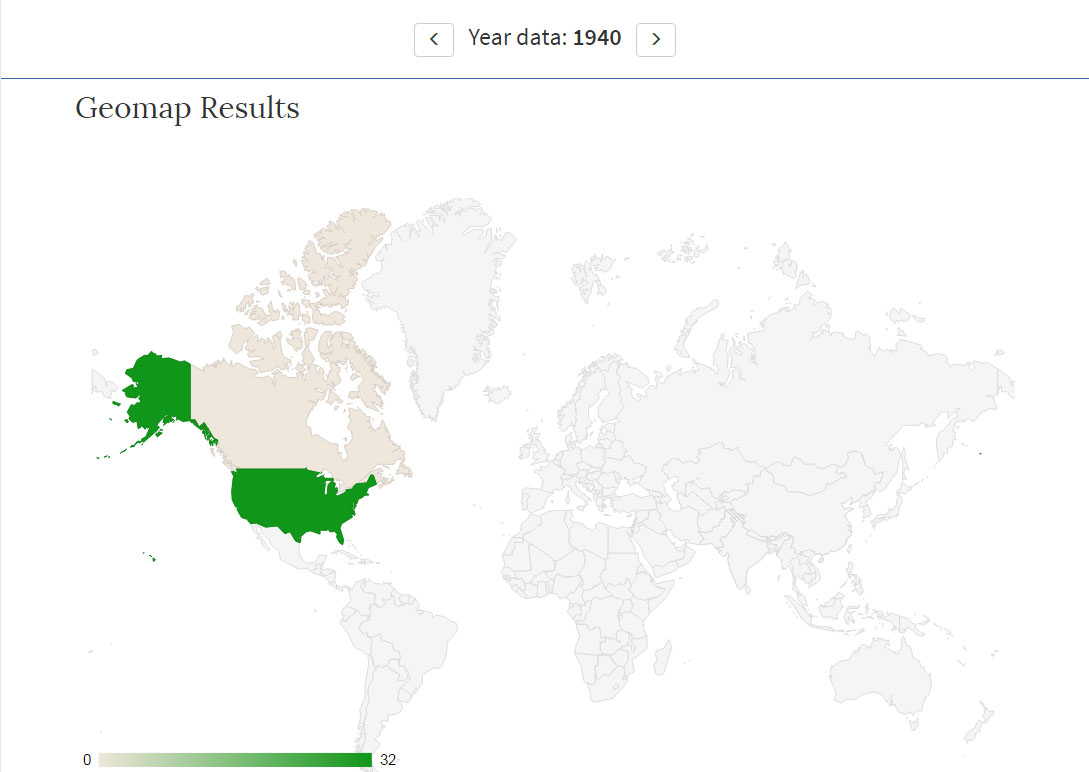
\includegraphics[width=\linewidth]{11/03_surnamesSearch/02_geomapDesktop}
    \centering
    \caption{Mapa geogràfic}\label{fig:geomap}
\end{figure}

\begin{figure}[h]
    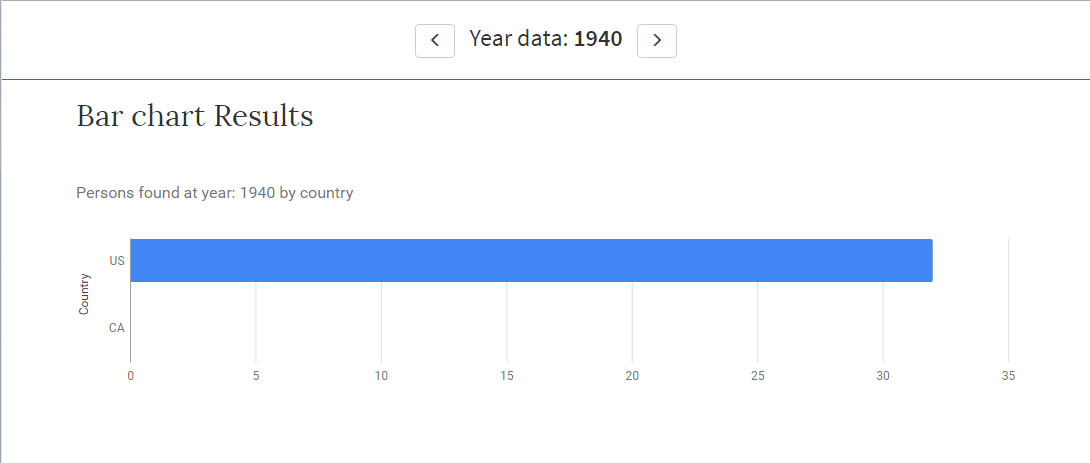
\includegraphics[width=\linewidth]{11/03_surnamesSearch/03_barChartDesktop}
    \centering
    \caption{Gràfic de barres}\label{fig:barchart}
\end{figure}

\begin{figure}[h]
    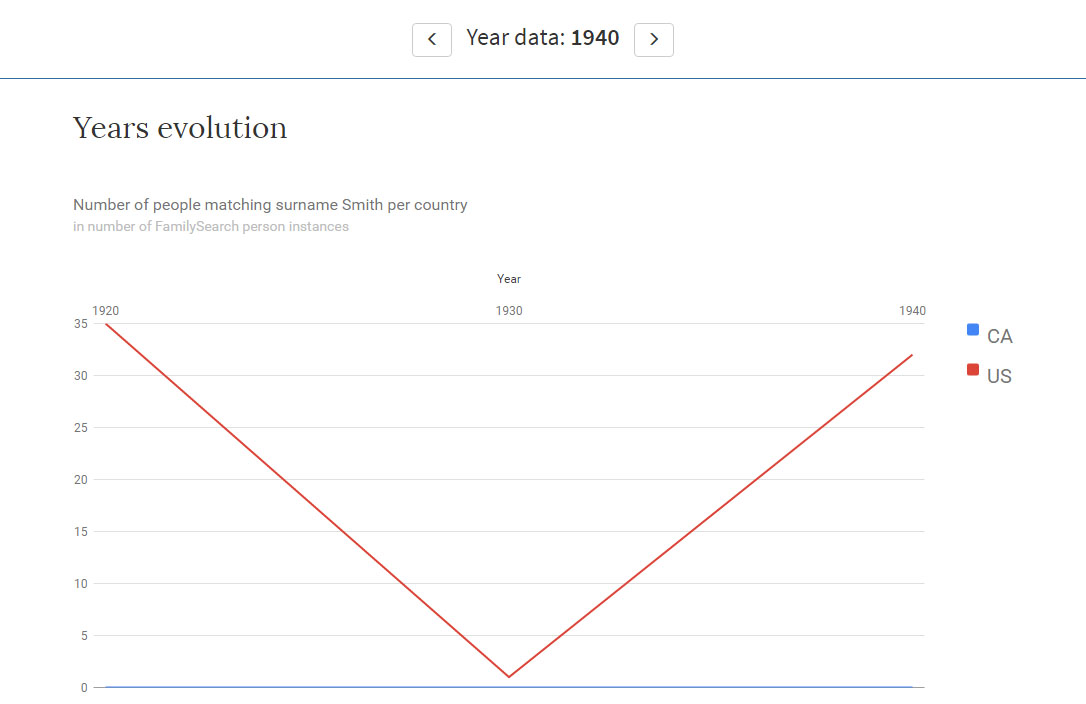
\includegraphics[width=\linewidth]{11/03_surnamesSearch/04_yearsEvolutionDesktop}
    \centering
    \caption{Gràfic de línies}\label{fig:linechart}
\end{figure}

